\documentclass[xcolor=table]{beamer}
\usepackage{subfig}
\usepackage{bytefield}
\usepackage[cache=false]{minted}
\usepackage[tikz]{bclogo}
\usetheme{metropolis}
\title{Wireguard: A Modern VPN Protocol}
\author{Jinank Jain, Rayhaan Jaufeerally}
\institute{Network Security Group, ETH Z\"urich}
\begin{document}
    \maketitle
    \section{Introduction}
    \begin{frame}{Why VPN?}
        \begin{itemize}
            \item Necessary for point to point security between campuses (e.g. DC's, corporate offices, \ldots)
                \begin{itemize}
                    \item As early as the 1970's governments have tapped undersea cables for intelligence,
                    \item Operation Ivy Bells in 1971 tapped Russian communications to military bases\footnote{\url{https://en.wikipedia.org/wiki/Operation\_Ivy\_Bells}},
                \end{itemize}
            \item Necessary for end users to get a clean connection:
                \begin{itemize}
                    \item ISP's doing DNS hijacking to serve inappropriate content,
                    \item Open WiFi networks when traveling,
                    \item Geoblocking,
                \end{itemize}
        \end{itemize}
    \end{frame}
    \begin{frame}{Necessity in real life}
        \begin{figure}
            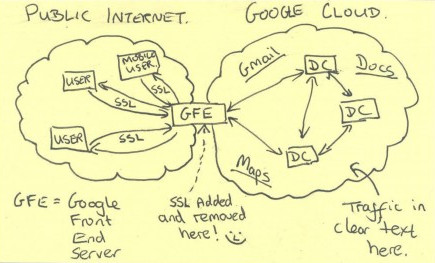
\includegraphics[width=\textwidth]{motivation.jpg}
            \caption{Nation state surveillance of user data including SPII.}
        \end{figure}
    \end{frame}
    \begin{frame}
        \begin{figure}
            \includegraphics[height=\textheight]{fstap.png}
            \caption{Common off the shelf fiber tap.}
        \end{figure}
    \end{frame}
    \begin{frame}{History of VPN protocols}
        \begin{itemize}
            \item IPSEC
                \begin{itemize}
                    \item Popular for site to site connections with dedicated router hardware,
                    \item Tedious to set up and high degree of complexity,
                    \item Large attack surface between IKE (v2), SA mechanisms, XFRM in Linux,
                    \item Legacy protocol support,
                    \item IP in IP,
                \end{itemize}
            \item OpenVPN
                \begin{itemize}
                    \item Implemented in userspace with TUN/TAP (slow),
                    \item Complex configuration vulnerable to leaks,
                    \item Stateful protocol which is brittle in real networks,
                    \item Large codebase / attack surface,
                \end{itemize}
        \end{itemize}
    \end{frame}
    \begin{frame}{What is Wireguard?}
        \begin{itemize}
            \item Opinionated Layer 3 secure network tunnel for IPv4 and IPv6.
            \item Lives in the Linux kernel, but cross platform userspace implementations are available.
            \item UDP based. Punches through firewall.
            \item Conservative and modern cryptographic principles.
            \item Emphasis on simplicity and single user auditability.
            \item Authentication model similar to SSH's \texttt{authorized\_keys}.
        \end{itemize}
    \end{frame}
    \begin{frame}{Easily Auditable}
        \begin{figure}
            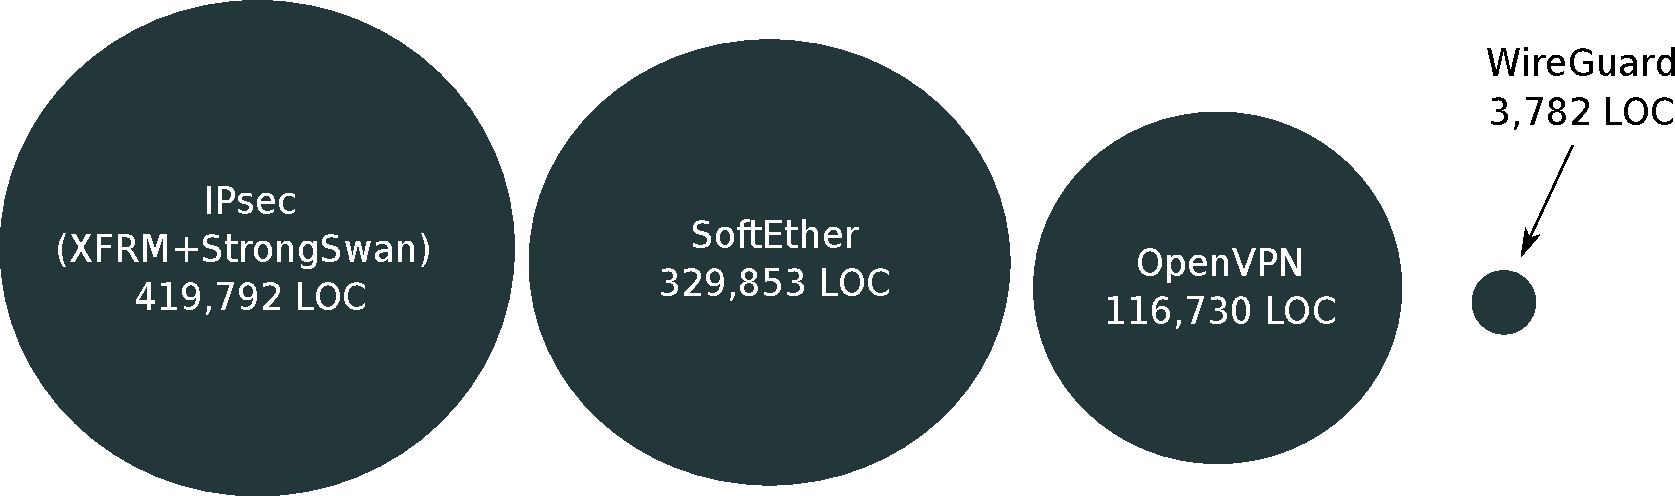
\includegraphics[width=\textwidth]{vpn_compare.pdf}
            \caption{Comparing different VPN protocols in terms of LOC}
        \end{figure}
    \end{frame}
    \begin{frame}[fragile]{Minimalistic Interface}
    ``Developers should write programs that can communicate easily with other programs''
    \\[5pt]
    \rightline{{\rm --- Unix Philosophy}}
        \begin{itemize}
            \item Wireguard presents a normal network interface
                \begin{minted}{shell}
ip link add wg0 type wireguard
ip address add 10.0.32.1/24 dev wg0
ip route add default via wg0
                \end{minted}
            \item By using a standard interface it becomes easier to administer using the existing iproute2 utilities for example
        \end{itemize}
    \end{frame}
    \begin{frame}{Cryptokey Routing}
        \begin{itemize}
            \item Fundamental concept of any VPN service
                \begin{itemize}
                    \item Create \textbf{mapping} between \textbf{public keys of peers} and their \textbf{IPs}.
                \end{itemize}
            \item WireGuard interface has:
                \begin{itemize}
                    \item A private key
                    \item A listening UDP port
                    \item A list of peers
                \end{itemize}
            \item Peer has
                \begin{itemize}
                    \item A public key
                    \item A list of associated tunnel IPs
                    \item Optionally has an endpoint IP and port
                \end{itemize}
        \end{itemize}
    \end{frame}
    \begin{frame}[fragile]{Cryptokey Routing}
        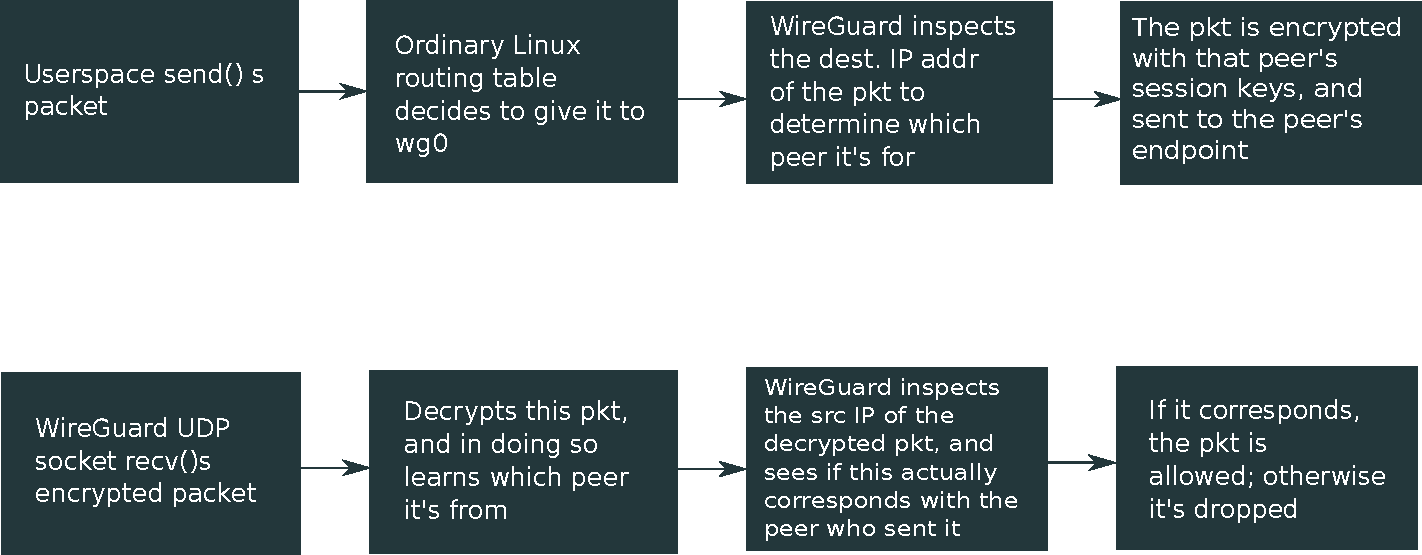
\includegraphics[width=\textwidth]{crypto_route.pdf}
    \end{frame}

    \section{Protocol design}

     \begin{frame}{Stealth}
        \begin{minipage}{0.6\textwidth}
            \begin{itemize}
                \item Behaves like a rootkit in some sense.
                \item Should not respond to any unauthenticated packets.
                \item Hinder scanners and service discovery.
                \item Service only responds to packets with correct crypto.
                \item Not chatty at all.
            \end{itemize}
        \end{minipage}
        \begin{minipage}{0.37\textwidth}
            \begin{figure}
                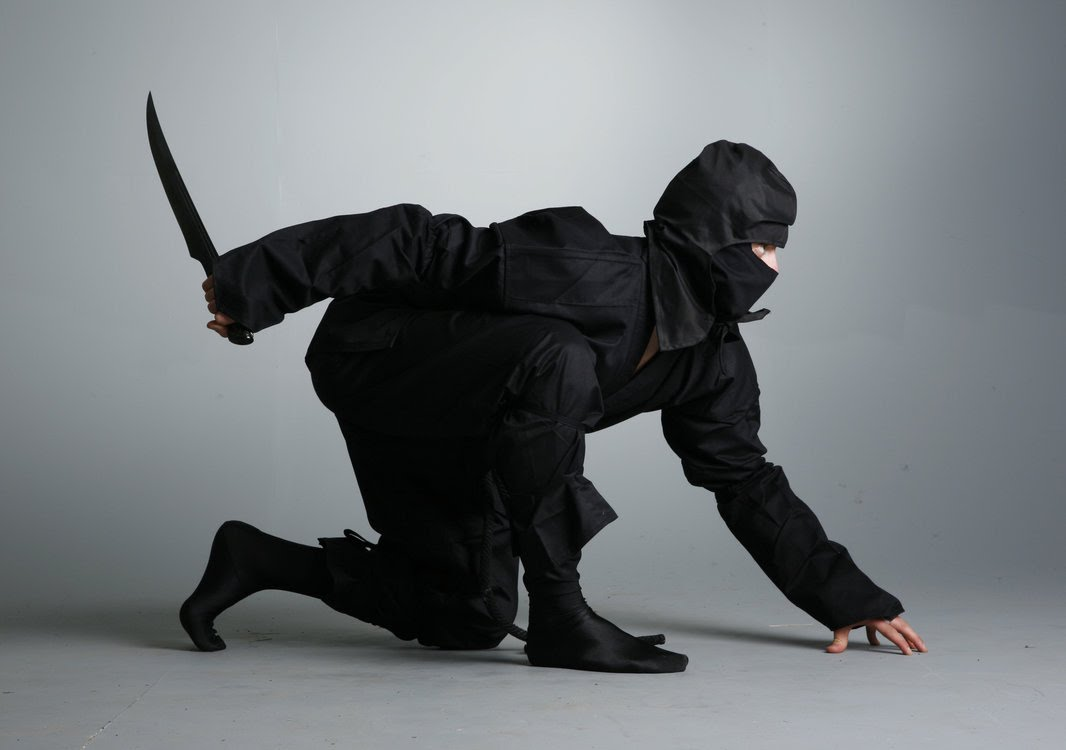
\includegraphics[width=\textwidth]{ninja.jpg}
            \end{figure}
        \end{minipage}
    \end{frame}

    \begin{frame}{Handshake DoS}
    \begin{itemize}
        \item Verifying authenticity using Curve25519 is expensive,
        \item Under load a responder may send a cookie which needs to be echoed back,
        \item This proves IP ownership, hence IP rate limiting can be used (e.g. token bucket).
        \item The cookie is the MAC over the source IP with a secret which changes every 120s.
    \end{itemize}
    \end{frame}

    \begin{frame}{Flaws to be addressed}
        \begin{itemize}
            \item Indiscriminate cookie responses violate silence property,
            \item Cleartext cookies are vulnerable to MiTM replay attacks which cause extra computation,
            \item Initiator itself could be DoS'ed by being sent fake cookies
        \end{itemize}
    \end{frame}

    \begin{frame}{Issue 1: Silence}
        \begin{itemize}
            \item For the responder to remain silent, all messages have a first MAC using the responder's public key,
            \item This proves that a peer knows to whom it is talking,
            \item While this public key is not secret, it is acceptable in the threat model to say if the initator knows the public key, then it knows of the existence of the responder,
            \item This MAC is included in all packets as \texttt{msg.mac1}
        \end{itemize}
    \end{frame}

    \begin{frame}{Issue 2: Cleartext cookies}
    \begin{itemize}
        \item The cookie is encrypted using \texttt{XChaCha20Poly1305 AEAD} with a randomized nonce,
        \item This uses the responder's public key as symmetric encryption key
    \end{itemize}
    \end{frame}

    \begin{frame}{Issue 3: Fraudulent cookies}
    \begin{itemize}
        \item The additional data field of AEAD to encrypt the cookie in transit is used to authenticate the first MAC,
        \item An attacker without an active MiTM cannot send fraudulent invalid cookie responses to prevent them from authenticating,
        \item This is acceptable in the threat model because a Dolev-Yao attacker could just drop packets to prevent authentication
    \end{itemize}
    \end{frame}

    \begin{frame}{Crypto background --- ChaCha20}
        \begin{itemize}
            \item A stream cipher designed by DJB based upon Salsa20,
            \item Uses simple operations: XOR, 32 bit addition mod \(2^{32}\), and constant distance rotation operations (\(<<<\)),
            \item Limiting to these instructions aims to avoid timing side channels,
            \item Internal state consists of sixteen 32-bit words in a \(4 \times 4\) matrix
        \end{itemize}
    \end{frame}

    \begin{frame}{Crypto background --- ChaCha20 State}
        \begin{table}
        \begin{tabular}{|c|c|c|c|}
            \hline
            \rowcolor{yellow!25}Cons & Cons & Cons& Cons\\
            \hline
            \rowcolor{blue!25} Key & Key & Key & Key\\
            \hline
            \rowcolor{blue!25} Key & Key & Key & Key\\
            \hline
            \cellcolor{red!25} Pos & \cellcolor{red!25} Pos & \cellcolor{green!25} Nonce & \cellcolor{green!25} Nonce\\
            \hline
        \end{tabular}
        \caption{Initial state of ChaCha20}
        \end{table}

        Constant used is ``expand 32-byte k'' which is a ``nothing up my sleeve number''.
    \end{frame}

    \begin{frame}[fragile]{Crypto background --- ChaCha20}
        \begin{minted}{c}
#define ROT(a,b) (((a) << (b)) | ((a) >> (32 - (b))))
#define QR(a, b, c, d)       \
   a += b;  d ^= a;  d = ROT(d,16);  \
   c += d;  b ^= c;  b = ROT(b,12);  \
   a += b;  d ^= a;  d = ROT(d, 8);  \
   c += d;  b ^= c;  b = ROT(b, 7)
        \end{minted}
    \end{frame}

    \begin{frame}[fragile]{Crypto background --- ChaCha20}
        \begin{minted}[fontsize=\footnotesize]{c}
void chacha_block(uint32 out[16],uint32 in[16]) {
  int i; uint32 x[16];
  for (i = 0;i < 16;++i) x[i] = in[i];
  // 10 loops x 2 rounds/loop = 20 rounds.
  for (int i = 0; i < 10; i++) {
    // Odd round.
    QR(x[0], x[4], x[ 8], x[12]); // column 0
    QR(x[1], x[5], x[ 9], x[13]); // column 1
    QR(x[2], x[6], x[10], x[14]); // column 2
    QR(x[3], x[7], x[11], x[15]); // column 3
    // Even round.
    QR(x[0], x[5], x[10], x[15]); // diagonal 1 (main diagonal)
    QR(x[1], x[6], x[11], x[12]); // diagonal 2
    QR(x[2], x[7], x[ 8], x[13]); // diagonal 3
    QR(x[3], x[4], x[ 9], x[14]); // diagonal 4
  }
  for (i = 0;i < 16;++i) out[i] = x[i] + in[i];
}
        \end{minted}
    \end{frame}

    \begin{frame}{Primitives}
    \begin{description}
        \item[DH(pubkey, privkey)] --- Curve25519 point multiplication of \texttt{privkey} and \texttt{pubkey}, 32 bytes output,
        \item[DH\_Generate()] --- Generates a random Curve25519 private key and computes its corresponding public key,
        \item[AEAD(key, counter, plaintext, authtext)] --- \texttt{ChaCha20Poly1305 AEAD} as specified in RFC 7539 with the nonce being 32 bits of zeros followed by 64bit LE value of \texttt{counter},
        \item[XAEAD(key, nonce, plaintext, authtext)] --- \texttt{XChaChaPoly1305 AEAD} with 24 byte random \texttt{nonce} instantiated using \texttt{HChaCha20} and \texttt{ChaChaPoly1305}
    \end{description}
    \end{frame}

    \begin{frame}{Primitives (cont'd)}
        \begin{description}
            \item[Hash(input)] --- \texttt{blake2s(input, 32)}
            \item[MAC(key, input)] --- \texttt{keyed-blake2s(key, input, 16)}, the keyed MAC variant of the BLAKE2s hash function, 16 byte output,
            \item[HMAC(key, input)] --- \texttt{HMAC-blake2s(key, input, 32)}, the ordinary BLAKE2s hash function used in an HMAC construction,
            \item[$\mathbf{KDF_n}$(key, input)] --- Sets \(\mathcal{T}_0 := HMAC(key, input), \mathcal{T}_1 := HMAC(\mathcal{T}_0, 0x1), \ldots, \mathcal{T}_i := HMAC(\mathcal{T}_0, \mathcal{T}_{i - 1} || i)\)
            \item[Timestamp()] --- Returns the TAI64N timestamp of the current time, 12 bytes output, first 8 bytes UNIX timestamp, last 4 bytes number of nanoseconds from the beginning of that second
        \end{description}
    \end{frame}

    \begin{frame}{The Key Exchange}
        \begin{figure}
            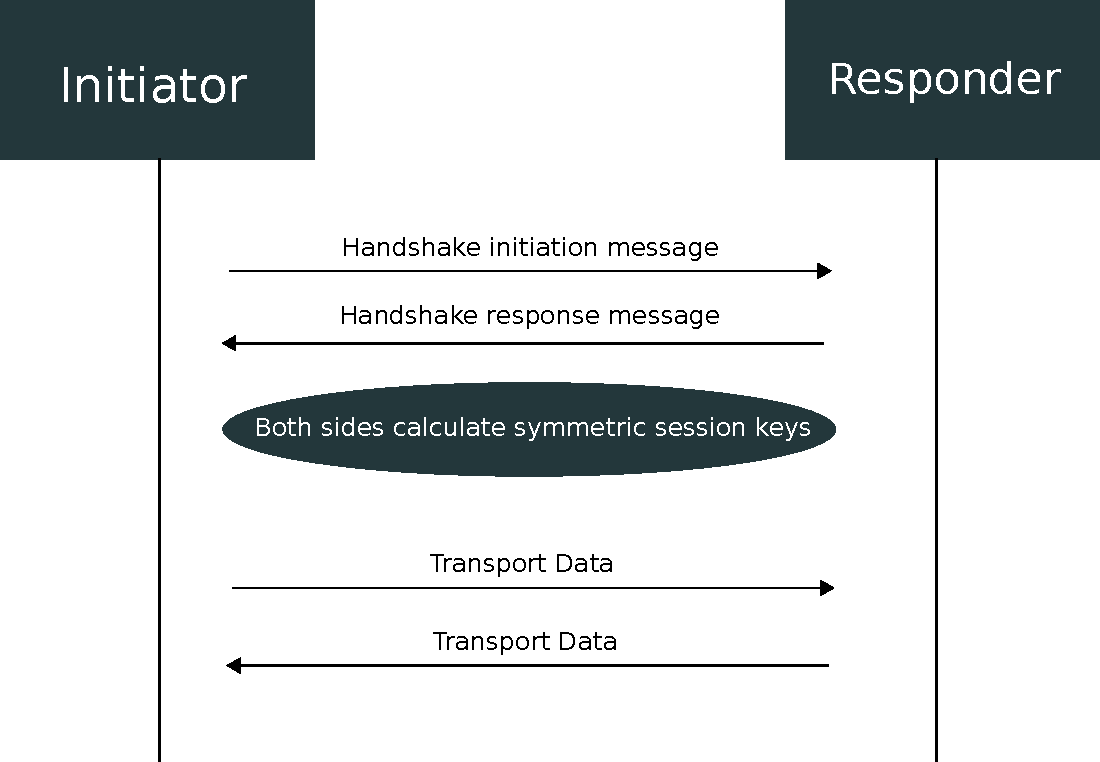
\includegraphics[width=\textwidth]{handshake.pdf}
        \end{figure}
    \end{frame}
    \begin{frame}{Session key derivation - NoiseIK}
        \begin{itemize}
            \item One peer is the initiator; the other is responder
            \item Each peer has their static identity - their long term \textit{static keypair}
            \item For each new handshake, each peer generates an \textit{ephemeral keypair}
            \begin{figure}
                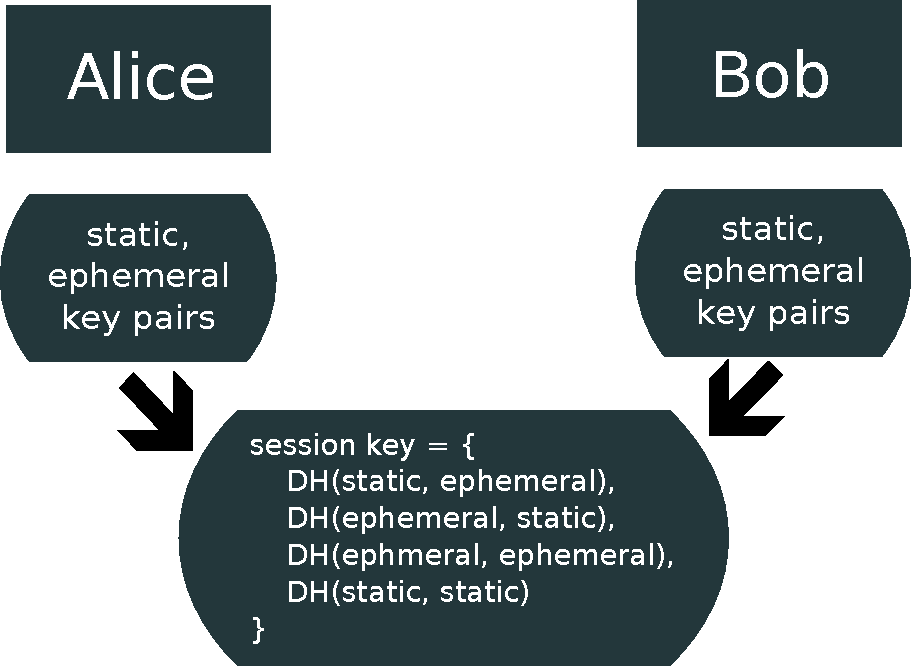
\includegraphics[width=0.6\textwidth]{session_key.pdf}
            \end{figure}
        \end{itemize}
    \end{frame}

    \begin{frame}{Message 1: Initiator to responder}
        %XXX Horrific abuse of bytefield to make it look nice.
        \begin{figure}
        \begin{bytefield}{32}
            \bitbox{13}{Type := 1 (1 byte)}
            \bitbox{19}{Reserved := 0 (3 bytes)}\\
            \bitbox{32}{Sender := $I_i$ (4 bytes)}\\
            \wordbox{1}{Ephemeral (32 bytes)}\\
            \wordbox{1}{Static (32 bytes)}\\
            \wordbox{1}{Timestamp (12 bytes)}\\
            \bitbox{16}{mac1 (16 bytes)}
            \bitbox{16}{mac2 (16 bytes)}
        \end{bytefield}
        \caption{Initator to responder packet. \tiny{\textsc{not to scale}}.}
        \end{figure}
    \end{frame}

    \begin{frame}{Message 1: computation}
        \begin{align}
            C_i &:= HASH(CONSTRUCTION)\\
            H_i &:= HASH(C_i~||~IDENTIFIER)\\
            H_i &:= HASH(H_i~||~S_r^{pub})\\
            (E_i^{priv}, E_i^{pub}) &:= DH\_generate()\\
            C_i &:= KDF_1(C_i, E_i^{pub})\\
            \mathtt{msg.ephemeral} &:= E_i^{pub}\\
            H_i &:= HASH(H_i~||~\mathtt{msg.ephemeral})\\
            (C_i, \kappa) &:= KDF_2(C_i, DH(E_i^{priv}, S_r^{pub}))\\
            \mathtt{msg.static} &:= AEAD(\kappa, 0, S_i^{pub}, H_i)\\
            H_i &:= HASH(H_i~||~\mathtt{msg.static})
        \end{align}
    \end{frame}

    \begin{frame}{Message 1: computation (cont'd)}
        \begin{align}
            (C_i, \kappa) &:= KDF_2(C_i, DH(S_i^{priv}, S_r^{pub})\\
            \mathtt{msg.timestamp} &:= AEAD(\kappa, 0, Timestamp(), H_i)\\
            H_i &:= HASH(H_i~||~\mathtt{msg.timestamp})
        \end{align}
    \end{frame}
    \setcounter{equation}{0}

    \begin{frame}{Message 2: Responder to initiator}
        \begin{figure}
        \begin{bytefield}{32}
            \bitbox{13}{type := 0x2 (1 byte)}
            \bitbox{19}{reserved := 0 (3 bytes)}\\
            \bitbox{16}{sender := $I_r$ (4 bytes)}
            \bitbox{16}{receiver := $I_i$ (4 bytes)}\\
            \wordbox{1}{Ephemeral (32 bytes)}\\
            \wordbox{1}{Empty (0 bytes)}\\
            \bitbox{16}{mac1 (16 bytes)}
            \bitbox{16}{mac2 (16 bytes)}\\
        \end{bytefield}
        \caption{Responder to initiator packet. \tiny{\textsc{not to scale}}}
        \end{figure}
    \end{frame}

    \begin{frame}{Message 2: computation}
        \begin{align}
            (E_r^{priv}, E_R^{pub}) &:= DH\_Generate()\\
            C_R &:= KDF_1(C_r, E_r^{pub})\\
            \mathtt{msg.ephemeral} &:= E_r^{pub}\\
            H_r &:= HASH(C_r~||~\mathtt{msg.ephemeral})\\
            C_r &:= KDF_1(C_r, DH(E_r^{priv}, E_i^{pub}))\\
            C_r &:= KDF_1(C_r, DH(E_r^{priv}, S_i^{pub})\\
            (C_r, \mathcal{T}, \kappa) &:= KDF_3(C_r, Q)\\
            H_r &:= HASH(H_r~||~\mathcal{T})\\
            \mathtt{msg.empty} &:= AEAD(\kappa, 0, \epsilon, H_r)\\
            H_r &:= HASH(H_r, \mathtt{msg.empty})
        \end{align}
    \end{frame}

    \begin{frame}{Transport data messages}
        \begin{figure}
         \begin{bytefield}{32}
            \bitbox{13}{type := 0x4 (1 byte)}
            \bitbox{19}{reserved := 0 (3 bytes)}\\
            \wordbox{1}{receiver := $I_{m'}$ (4 bytes)}\\
            \wordbox{1}{counter (8 bytes)}\\
            \wordbox[lrt]{1}{packet data}\\
            \skippedwords\\
            \wordbox[lrb]{1}{}\\
        \end{bytefield}
        \caption{Payload packet. \tiny{\textsc{not to scale}}}
        \end{figure}
    \end{frame}
    \begin{frame}{Timers: A Stateless Interface for a Stateful Protocol}
        \begin{itemize}
            \item Wireguard appears "\textbf{stateless}" to userspace; you set up peers, and then it just works.
            \item Series of timers manages session state internally, invisible to the user.
            \item Every transition of the state machine has been accounted for, so there is no undefined states or transitions.
            \item Event based.
        \end{itemize}
    \end{frame}
    \begin{frame}{Timers}
        \begin{bclogo}[logo = \bchorloge, arrondi = 0.1]{Userspace sends packets.}
        If no session has been established for 120 seconds, send handshake initiation.
        \end{bclogo}
        \begin{bclogo}[logo = \bchorloge, arrondi = 0.1]{No handshake response after 5 seconds.}
        Resend handshake initiation.
        \end{bclogo}
        \begin{bclogo}[logo = \bchorloge, arrondi = 0.1]{Successful authentication of incoming packet}
        Send an encrypted packet after 10 seconds, if we don't have anything else to send during that time.
        \end{bclogo}
        \begin{bclogo}[logo = \bchorloge, arrondi = 0.1]{No successfully authenticated
incoming packets after 15 seconds.}
        Send handshake initiation.
        \end{bclogo}
    \end{frame}
    \begin{frame}[fragile]{Performance}
        \begin{figure}
            \hspace*{-1cm} \subfloat{{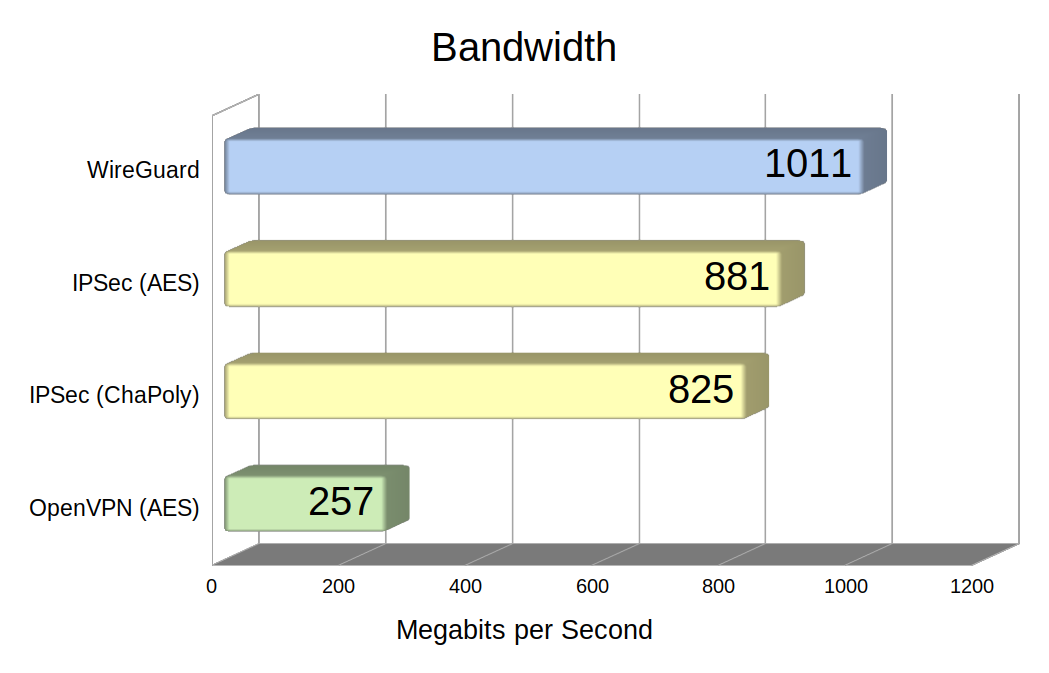
\includegraphics[width=6cm]{bandwidth.png} }}%
            \subfloat{{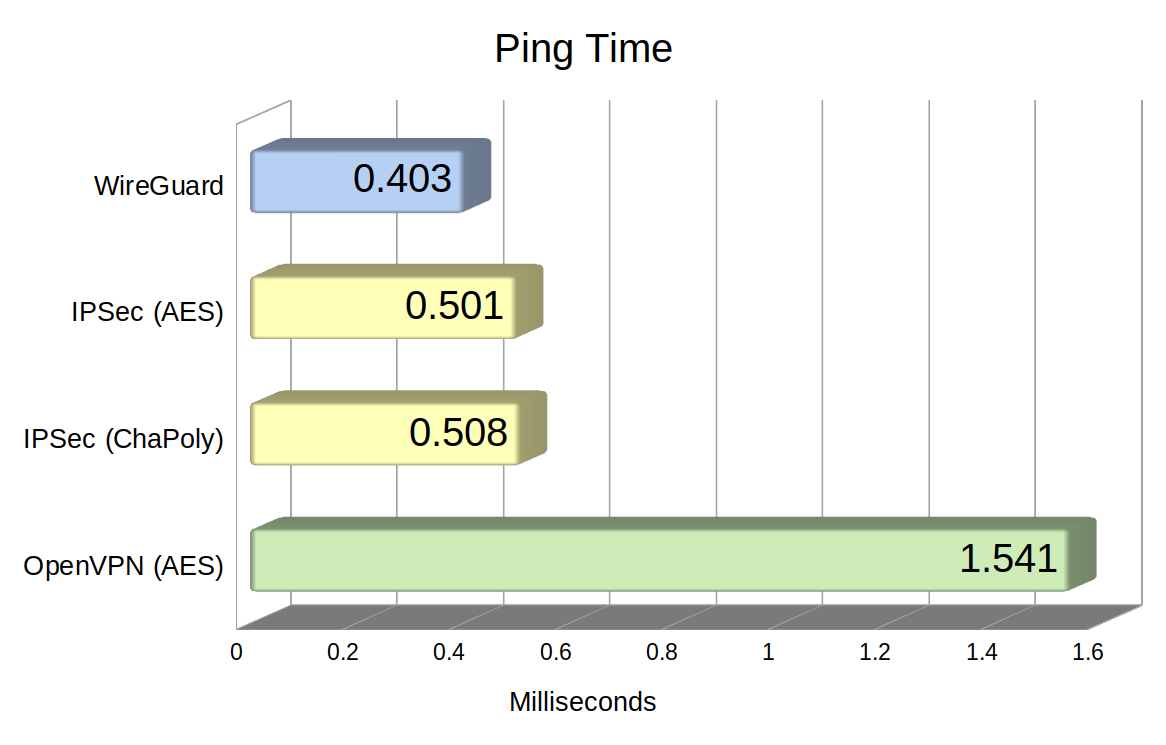
\includegraphics[width=6cm]{ping.png} }}%
            \label{fig:example}%
        \end{figure}
    \end{frame}
    \begin{frame}{Recap}
        \begin{minipage}{0.48\textwidth}
            \begin{itemize}
                \item Less than 4,000 lines of code
                \item Easily implemented with basic data structures
                \item Minimal state kept, no dynamic allocations
                \item Solid cryptographic foundation.
            \end{itemize}
        \end{minipage}
        \begin{minipage}{0.5\textwidth}
            \begin{itemize}
                \item Extremely performant - best in class.
                \item Stealthy and minimal attack surface
                \item Simple standard interface via an ordinary network device.
                \item Opinionated.
            \end{itemize}
        \end{minipage}
    \end{frame}
    \begin{frame}[fragile]{Install instructions}
        \begin{itemize}
            \item Ubuntu
            \begin{minted}{shell}
sudo add-apt-repository ppa:wireguard/wireguard
sudo apt-get update
sudo apt-get install wireguard
            \end{minted}
            \item macOS
            \begin{minted}{shell}
brew install wireguard-tools
            \end{minted}
        \end{itemize}
    \end{frame}
\end{document}
